\documentclass[11pt]{article}
\usepackage{deauthor}
\usepackage{graphicx}
\usepackage{graphicx}
\usepackage{times}
\usepackage{subfig}
\usepackage{makecell}

%\usepackage[driverfallback=dvipdfm]{hyperref}

\newcommand\keywords[1]{\textbf{Keywords}: #1}

\begin{document}

\title{A Perspective Survey on Industrial Knowledge Graphs: Recent Advances, Open Challenges, and Future Directions}

\author{Yuhu Shang$^\dag$
\and
Hao Peng $^\ddag$ \thanks{Corresponding authors.}
\and
Yimeng Ren$^\dag$
\and
Yue Wang $^\ddag$
\and
Gang Wang $^\S$
\and
Zhongcheng Li $^{\ss}$
\ \ \ \ \ \
Yifeng Liu $^\P$
\ \ \ \ \ \
Yangyang Li $^\P$ $^\|$  \footnotemark[1]
\\
$^\dag$ Tianjin University of Science \& Technology, China \ \ \
\normalsize{\{shangyhhu6902, renyimeng\}@mail.tust.edu.cn}
\\
$^\ddag$ Beihang University, China \ \ \ \normalsize{\{penghao, zb2039111\}@buaa.edu.cn}
\\
$^\S$ Beijing Institute of Technology, China \ \ \ \normalsize{gangwang@bit.edu.cn}
\\
$^{\ss}$ China Tower Corporation Hebei Branch, China \ \ \ \normalsize{lizc@chinatowercom.cn}
\\
$^\P$ National Engineering Research Center for Risk Perception and Prevention, China \\ \normalsize{liuyifeng3@cetc.com.cn}
\\
$^\|$ Academy of Cyber, China \ \ \ \normalsize{liyangyang@cetc.com.cn}
}
\maketitle
\begin{abstract}
As a result of the development of a new generation of artificial intelligence and carbon-neutral technologies, traditional industry is undergoing dramatic transformations.
Industry's exploration of industrial intelligence is still in its early stages.
There is a particular lack of technical means for condensing empirical knowledge from multiple sources of heterogeneous data.
Knowledge Graphs (KG), as cutting-edge artificial intelligence technologies, can enable knowledge management and reuse while condensing knowledge.
As a result, fully utilizing KG's potential in the industrial field is critical to the realization of autonomous sensing, cognition, and the evolution of next-generation intelligent manufacturing systems.
Starting with the current state of industrial knowledge graph development, the paper shows how to construct an industrial knowledge graph (IKG).
Following that, we provide a thorough and in-depth review of industrial knowledge graph construction methods applied to various scenarios.
We summarize the existing industrial knowledge graph construction approaches and compare them in terms of technical components and characteristics.
Then, we categorize the knowledge graph-supported application scenarios, which include predictive maintenance, fault diagnosis, interpretable knowledge recommendation, industrial safety, intelligent decision making, and production efficiency.
Furthermore, this paper identifies the current challenges confronting industrial applications and proposes future research directions for IKG.
It is hoped that this research will draw the attention of more researchers to the knowledge graph-based smart manufacturing paradigm and benefit their work.
\end{abstract}


\section{Introduction}

\par{Intelligent manufacturing technologies have been driven by the rapid development of artificial intelligence, industrial internet, edge computing, and other emerging information technologies.
Countries all over the world have identified the development of a new generation of intelligent manufacturing technology as a critical technology for increasing global competitiveness.
Intelligent manufacturing systems have initially possessed basic capabilities such as state monitoring and auxiliary decision-making following recent development.
However, there are still flaws, such as an over-reliance on human intervention and difficulty completing complex tasks on one's own.
This is because current intelligent manufacturing systems are incapable of summarizing and summarizing empirical knowledge in the same way that humans do.
}

\par{KG is an artificial intelligence technology that manages, coordinates, and distills all types of knowledge (e.g. mechanism, experience, data, etc.) \cite{bib1}.
By organizing massive heterogeneous concepts with interconnected nodes and defining cross-level relationships with heterogeneous edges, knowledge graph can aid intelligent manufacturing systems in their ability to acquire and deduce detailed knowledge \cite{bib2}.
When constructing industrial knowledge graph (IKG), strategies such as multiple views are commonly used to define the attribute characteristics of the connected edges of heterogeneous nodes\cite{bib3}.
This type of processing becomes a powerful support for the downstream tasks of intelligent manufacturing systems.
Such technologies as predictive maintenance, total supply chain optimization, and digital twins all benefit from the support of industrial knowledge graphs.
By providing support for industrial intelligence, knowledge graph technology not only promotes the development of the industrial sector, but also improves the quality of production and service.
In conclusion, the incorporation of knowledge graph technology into the industrial sector is critical for industrial intelligence.}


\par{\textbf{Related Surveys and Our Contributions.}
In recent years, the critical review of KG applications in industrial scenarios has attracted surging attention.
For instance, the authors of \cite{bib4} particularly analyzed potential applications of KGs in scenarios and mainly focused on maintenance, optimization, and resource allocation.
Studies related to KG for Industry 4.0 modeling standards, norms, and frameworks are reviewed in \cite{bib5}.
The work in \cite{bib6} provides a thorough review of industrial knowledge graphs, which presents its advantages, applications, and future perspectives.
By contrast, several surveys focus on different types of industrial scenarios, such as food science and industry \cite{bib7}, power transformers \cite{bib8}, intelligent decision-making \cite{bib9}, smart grid \cite{bib10}, fault diagnosis \cite{bib11}, underground pressure forecasting \cite{bibfo}, and furniture production \cite{bib12}.
Although there are several review articles with regard to the IKG topic, they do not provide a comprehensive summary of KG development, challenges, and future prospects in industrial products and services. }

\par{The key aim of this survey is to give a holistic overview of the recent development in industrial knowledge graphs, fully demonstrating the practicability of knowledge graph-driven technology in the industrial smart product service.
The main aspects of this review are as follows:}

\par{$\bullet$ We first revisit the various steps involved in the industrial knowledge graphs construction process.}

\par{$\bullet$ We systematically categorize the IKGs and divide the IKGs into predictive maintenance, fault diagnosis, explainable knowledge recommendation, industrial security, intelligent decision-making, and production efficiency topics.
We present several major works and their corresponding models for each topic.}

\par{$\bullet$ We further summarize some open challenges and future research directions of adopting knowledge graphs on the industrial manufacturing process.}


\par{The outline of this survey is arranged as follows.
Section \ref{sec2} describes the methodology of our work, including the selection and analysis of literature.
Section \ref{sec3} further presents a workflow for building knowledge graphs.
Section \ref{sec4} introduces the application of knowledge graph in industrial scenarios.
Sections \ref{sec5}, \ref{sec6} point out the limitations of knowledge graph in the field of intelligent industrial and the future directions.
Finally, conclusions are drawn in Section \ref{sec7}.}

\section{Selection and Description of Sources} \label{sec2}
\par{In this section, we described our taxonomy, which summarizes the results of our search process.
We follow certain criteria to search articles for more discussion in this review, and four renowned academic databases, namely, (1) IEEE, (2) Elsevier, (3) Springer, and (4) Association for Computing Machinery (ACM), are adopted to retrieve the related literature.
To restrict the conceptual boundaries, the search terms consist of the combinations of two groups of keywords.
The first group is about the KG-based deep learning techniques, e.g., ``knowledge graph", ``graph embedding", ``knowledge fusion", ``knowledge extraction", ``knowledge graph embedding", ``knowledge graph reasoning", ``knowledge graph representation", etc.
The second group is about the industrial environments as well as specific applications, e.g., ``industrial applications", ``industrial internet", ``industrial robot", ``predictive maintenance", ``fault diagnosis", ``recommendation", ``industrial safety", ``intelligent industrial decision-making", etc.
Then, to ensure that this review is up to date, only articles published online from 2013 to 2022 (accessed on 12/01/2022) were considered.
After that, we excluded articles that did not belong to industrial domains (e.g., biology).
Lastly, we have conducted a comprehensive analysis of these articles, reviewing their abstracts and contents and selecting a number of representative studies for discussion.
The final selection contains 68 related papers.}

\section{Building Industrial Knowledge Graphs}\label{sec3}
\par{In the context of the formal model regarding the construction of industrial knowledge graph can be categorized into three stages.
Hence, the IKG process can be enumerated as knowledge construction, representation and reasoning, and using stages.
Regardless of the implemented details, we cast them in a unified workflow as drawn in Fig. \ref{framework}.}


\begin{figure}[htbp]
	\centering
	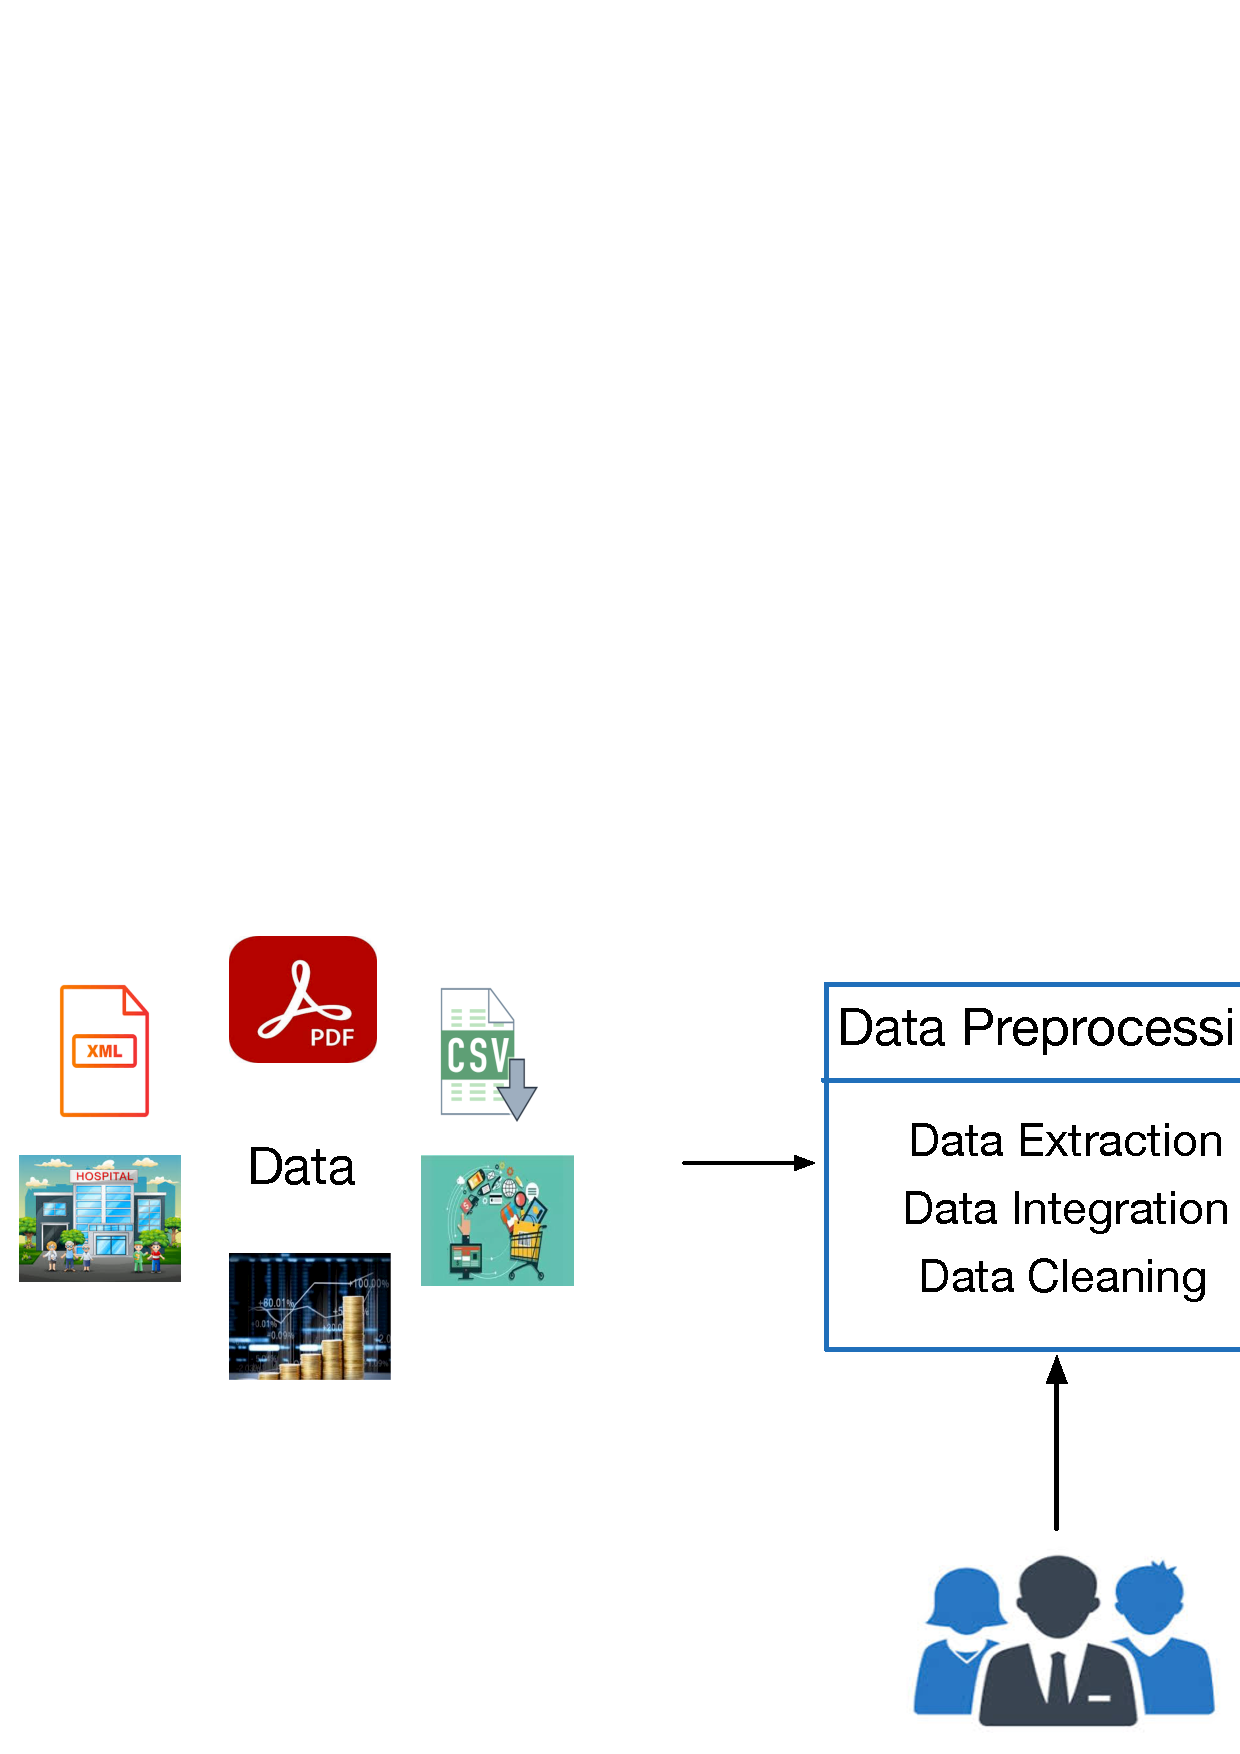
\includegraphics[width=0.7\linewidth]{submissions/industrial-kg/framework.pdf}
	\caption{A workflow for constructing and implementing industrial knowledge graphs.}
	\label{framework}
\end{figure}


\subsection{Knowledge Construction Stage}
\par{Raw data of industrial systems majorly exist in multiple heterogeneous data sources using different knowledge representations.
Therefore, the raw data in industrial scenarios have a lot of noisy facts in the knowledge construction stage.
Knowledge acquisition aims to acquire relevant entities, attributes, relations, rules, and facts from semi-structured and unstructured data in industrial scenarios.
To guarantee the high accuracy of acquired knowledge, some advanced natural language processing (NLP) and machine learning techniques were used in the construction stage.
Besides, some advanced deep learning methods such as LSTM-CRF, BiLSTM-CRF, BERT-BiLSTM-CRF, etc., which are also proposed to extract entities and indicate the dispatching behavior relationship patterns \cite{bib13}.
Knowledge fusion is an important technique to achieve the sharing, association, and discovery of knowledge units, and through this fusion, deliver new knowledge \cite{bib14}.
And its main processes include entity alignment and entity linking.
At the end of the knowledge construction stage, knowledge refinement can further detect noise in KGs to inconsistency checking and modify the knowledge graph adopting entity classification, relation prediction, and anomaly detection to improve the quality of the constructed knowledge graph \cite{bib15}.
Among the reviewed studies, Neo4j or FlockDB, are popular choices for building knowledge graphs and for modeling industrial data \cite{bib16}.
}


\subsection{Representation and Reasoning Stage}
\par{Effective knowledge representation learning methods should be explored based on the knowledge construction stage.
Learning low-dimensional distributed embedding of entities and relations is the core of representation learning.
In industrial scenarios, translation-based \cite{bib17} and tensor factorization-based \cite{bib18} models are classic; neural network-based \cite{bib19} methods occupy an important position in knowledge representation learning.
After the preliminary knowledge representation, the new information is obtained through knowledge reasoning\cite{bibsa}, including entity alignment and padding and attribute value alignment. Different reasoning methods, such as rule-based \cite{bib20}, distributed representation learning-based \cite{bib21}, and neural network-based \cite{bib22}, are proposed.}


\subsection{Using Stage}
\par{When knowledge systems are deployed into a real-world application, the primary concern of this stage is to enable stakeholders to manipulate the knowledge base without the need to know the details.
In recent years, many scholars have made unremitting explorations in this field.
For example, Jiang et al. \cite{bib23} implement a medical question-answering system and integrate medical professional knowledge.
Ren et al. \cite{bib24} developed a manufacturing knowledge graph, which extracts industry knowledge triples from different manufacturing field data.
Another aspect of the research is the design of a human-machine interface to present ergonomic characteristics, such as friendliness, usability, transparency, etc.
For instance, chatbots \cite{bib25}, visualized graphs \cite{bib26}, and question-answering systems \cite{bib27}, also prove their effectiveness in several industrial cases.
Currently, how to design and develop to meet the usability, flexibility, and economy of human-machine interfaces is still challenging.}


\section{An Overview of Knowledge Graphs Technology in Industrial Scenarios}\label{sec4}
\par{Due to the rich structured knowledge, knowledge graphs can be widely used in many downstream tasks.
However, how integrating such structured knowledge into the demand application of industrial scenarios remains a challenge.
Specifically, two subsects are included in knowledge graph application: 1) in-IKG applications, such as fault diagnosis and predictive maintenance, and 2) out-of-IKG applications, including intelligent decision-making and more downstream knowledge-aware applications, such as explainable knowledge recommendation and industrial security.}


\subsection{Predictive Maintenance}
\par{Predictive maintenance is a preventive maintenance approach for developing a more sustainable, safe, and profitable industry.
It is performed based on an online health assessment and predicts the breakdown of the system to be maintained by detecting early signs of failure.
Some researchers \cite{bib29} adopted industrial maintenance methods to decrease the delay in smooth operations, i.e., reduce machines or systems outages and unplanned downtime.
The predictive maintenance methods can be mainly categorized into three types: 1) model-based prognosis, 2) knowledge-based prognosis, and 3) data-driven prognosis.
Over the past few years, data-driven predictive maintenance technology has attracted wide interest.
For example, the work in \cite{bib30} thoroughly describes the applications of deep learning algorithms in rotary machinery systems, such as predictive maintenance, health management, and diagnosis decision, among others.
In the latest relevant research, the author in \cite{bib31} developed an intelligent data-driven predictive maintenance system through the Adabelief-BP method.
Applications show that this system can be implemented to automate the predictive maintenance process.
Umeda et al. \cite{bib32} identified maintenance plans that should incorporate additional predictive maintenance work by considering the probabilistic variability of predicted failure times.
Yu et al. \cite{bib33}] developed a big data ecosystem to implement fault detection in predictive maintenance. }

\subsection{Fault Diagnosis}
\par{Fault diagnosis (FD) serves a critical role in exploring the relationship between the monitoring data and the health status of machines, which has been a widely concerned issue in industrial products and services.
Many researchers have proposed various methods to achieve the fault diagnosis of industrial scenarios, including the deep neural networks \cite{bib34}, kernel relative entropy \cite{bib35}.
It is worth mentioning that both academia and industry have done substantial research on the faults of transformer \cite{bib36}, circuit breaker \cite{bib37}, and pneumatic valve \cite{bib38} in industrial scenarios.
Besides, the statistic and nonstatistical data-driven methods are often utilized jointly.
For example, Cho et al. \cite{bib39} applied a Bayesian network and recurrent neural network to diagnose and isolate faults in induction motors.
The author in \cite{bib40} proposed a new model that integrates sparse auto-encoder (SAE) and support vector machine (SVM) for industrial fault diagnosis.
To provide information-rich and accurate fault-related knowledge, they first used a reinforcement learning (RL) \cite{bibts} technique to mine hidden semantic knowledge to complete the missing relation and then used the graph neural networks \cite{bib41} to compute the embedding vector of new entities outside for continuously completing missing entities. }



\subsection{Explainable Knowledge Recommendation}
\par{Knowledge recommendation can proactively fulfill multiple stakeholders' (e.g., the user, provider) needs in the engineering solution design process, thus assisting them in boosting the efficiency of related development activities.
Among the reviewed studies, the explainable recommendation promotes the development of multistakeholder research \cite{bib43}.
Under the engineering solution design scenario, providers whose products have low recommendation interpretability may experience low engagement and would lose trust in participating in a given system if they believed such a system did not provide a solid knowledge-based explanation.
Compared with the traditional KG methods, we believe that multiple paths in the knowledge graph can improve the recommendation results as well as provide interpretability \cite{bib44}.
Lin et al. \cite{bib45} introduced knowledge graph into intelligent development services and proposed a model, which considered the skill characteristics of developers and the potential collaborative relationship among them to boost the performance of software refactoring recommendations.}

\subsection{Industrial Security}
\par{The large-scale deployment of sensors in industrial systems brings significant security risks and challenges.
How to provide effective safety services has always been a hot topic in the industrial safety field.
In the context of industrial safety Inspection, Dorodnykh et al. \cite{bib46} proposed a method to automate the extraction of specific entities from tabular data to fill and expand the target knowledge graph and demonstrated the validity of the semantic interpretation of individual tabular elements as a key feature through a case study.
Fang et al.
\cite{bib47} designed a hybrid computer vision and ontology model to identify hazards from images automatically.
By using historical railway reports, Liu et al. \cite{bib48} integrated the deep learning network, and combined the data enhancement method to build a connected network of hazards and accidents to form a knowledge graph, which was applied to railway hazard identification and risk assessment, further assisted the formulation of railway risk preventive measures.
Meng et al. \cite{bib49} proposed a security-aware dynamic scheduling model for real-time resource allocation in industrial control systems.}


\subsection{Industrial Intelligent Decision-making}
\par{In the last few years, intelligent decision-making has become a hot topic in industrial scenarios and benefited many decision-making-related tasks and real-world applications across a variety of areas\cite{bibgk}, including food science, healthcare, and drug adverse reactions analysis. }

\par{\textbf{Food Science.}
In the food science and industry field, robot manipulators can monitor the food processing lines through smart sensors, and implement intelligent processing control based on the knowledge from food knowledge graphs \cite{bib50, bib51}.
Especially, the COVID-19 pandemic has increased the need to pay more attention to enhancing digitalization and automation in the food industry.}

\par{\textbf{Healthcare.}
Knowledge graph plays an increasingly important role in the healthcare domain due to their potential to furnish better knowledge inference and further support evidence-based clinical decision-making.
The smart healthcare system can extract health-related information and organize health knowledge that assists stakeholders ( e.g., doctors, patients, clinical and research centers) in decision-making \cite{bib52, bib53}.}

\par{\textbf{Drug Adverse Reactions Analysis.}
Based on numerous pieces of evidence, timely identification of adverse drug reactions has a significant impact on patient behavior.
Pham et al. \cite{bib54} proposed a dynamic knowledge graph to support adverse reactions analysis of the drug considering a higher number of features for drug modeling.
The work in \cite{bib55} underlines the necessity of building an industrial knowledge graph that can help practitioners and managers yield a solution that outperforms human decision.}


\subsection{Production Efficiency}
\par{The increasing information complexity and its influence on production efficiency are fundamentally crucial for current manufacturing processes \cite{bib56}.
Especially, production efficiency is the decisive factor determining enterprises' economic benefits.
A number of researchers have achieved remarkable progress in this issue.
To shorten the product development cycle, the work in \cite{bib57} developed a general system architecture of cloud-based manufacturing equipment that significantly promotes workshop production efficiency.
Zhou et al. \cite{bib58} explore the implicit relationship between complex engineering data through knowledge graph, it integrates the implicit engineering knowledge in a machining workshop environment and is used for supporting the optimization of resource allocation.
Additionally, industrial robots have also shown their superiorities in improving total factor productivity owing to the benefit of cost efficiency, high flexibility, and multi-functionality of industrial robots, such as Kragic et al. \cite{bib59}, Steinhauser et al. \cite{bib60}. }


\section{Open Challenges}\label{sec5}
\par{With the increasing application of knowledge graph, scholars have been striving to understand how to develop knowledge-driven intelligent manufacturing systems.
Although there has been some progress in industrial KG construction and application in the past decades, they are still affected by inherent limitations and technical bottlenecks.
Therefore, this section further presents some remaining challenges of adopting knowledge graphs on industrial scenarios.}

\subsection{Data Quality Requirements}
\par{The data quality of the practical industry significantly affects performance, but real industrial scenarios generally contain high levels of noise, sparsity, and complex heterogeneous data.
In this case, development activities driven by incomplete or noisy information may cause a system to crash or malfunction.
To address these issues, data cleaning, normalization, and knowledge fusion techniques should be performed to remove inconsistencies and boost the correctness, quality, and integrity of the data.
Besides, some studies attempted to introduce other novel knowledge curation mechanisms to measure KG completion, and KG correctness approaches \cite{bib61}, but the involvement of extra work is still unavoidable to meet the infrastructure requirements, which may consume a lot of resources and financial resources.
Therefore, being able to monitor and improve the data quality can open a wide range of possibilities to help their development in the IKG solution of practical application.}

\subsection{Huge Computing Burden}
\par{KG is currently well-performed in the industrial application scenarios, due to the high complexity of industrial manufacture production, constructing large-scale industrial KGs needs to process an enormous amount of training parameters hence how to efficiently solve the problem of high computation cost caused by massive parameter is a pain point that plagues the industrial application.
For example, condition monitoring of industrial robot gears can decrease unexpected downtimes of highly automated production lines and thus save related costs.
Due to expensive hardware, the implementation of such a solution is costly itself.
Therefore, to fully exploit KG’s advantages in industrial applications to better support low-cost industrial manufacture, the KG-industry interaction needs further enhancement.
In fact, we are convinced that the development of a low-cost, high-efficiency industrial automation technology will be a great advance in this sector.}


\subsection{Multi-line and Multi-product Constraints}
\par{In actual situations, industrial manufacturing production is a highly complex decision-making problem, a set of requirements and constraints ought to be considered, including preferable product line segment, resource sharing constraint, minimum run-length constraints, and so on.
To directly optimize multiple objectives, several existing methods \cite{bib62, bib63} adopt constraint optimization methods that reduce the loss of one objective when optimizing another.
However, the constraint optimization is optimized objective-by-objective, which is still time-consuming in the real production scheduling process.
Therefore, industrial manufacturing production requires solutions considering more objectives or constraints as many operations need to be executed for industrial scheduling processes.
Obviously, to accelerate the process of industrial manufacturing production, it is necessary to have better solutions for the optimization of production scheduling KG-based.}

\section{Future Perspectives}\label{sec6}


\par{Based on the exhaustive literature survey above, we assume that the following several aspects remain open: human-machine co-evolvement has attracted the attention of researchers in industrial knowledge graph due to their ability to explore the interaction between a human and a robot; explanations that are dynamic, to provide understandable human explanations on how they behave; research on multi-modal knowledge aggregation that addresses the needs discussed within the theses; and research on few-shot and zero-shot learning.}


\begin{figure}[htbp]
	\centering
	\includegraphics[width=0.7\linewidth]{submissions/industrial-kg/future_perspectives.pdf}
	\caption{Four future perspectives aiming to more practical IKG exploitations.}
	\label{future_perspectives}
\end{figure}

\subsection{Human-machine Co-evolvement}
\par{As a core value of forthcoming Industry 5.0, human-machine co-evolvement has gained significant interest in the industry community.
Human workers are good at tasks requiring high-level cognitive decision-making and exception handling.
Meanwhile, the machine needs to take more responsibility for supporting precise computing, high repeatability, and fast production.
We could construct to bridge the semantic gap by the knowledge graph and break human operators' thinking sets with creative insights discovered by the cognitive machines.
In this sense, it is necessary to design more effective and elegant models to proactively improve their performance in the manufacturing process.
Therefore, it is expected that in the coming years, develop a sophisticated mechanism in which humans and machines can mutually assist and evolve together for sustainable growth.}



\subsection{Interpretable DL Models}
\par{Although neural methods are good at scalability, they lack interpretability, and it is not convincing to understand how and why they can make the final decision.
This limits the application of the model in industrial products and services, as operation managers might not fully trust models lacking explanatory results.
The core idea of decision-making in engineering requires the outputs of models accompanied by scientific physical understanding.
Explanation illustrates the reliability of the decisions and acts as a driver to create a trustworthy solution.
Due to these aspects, the theory of interpretable machine learning has gained increasing interest in academic areas, and multiple models have been applied to handle this issue.
One straightforward way to do this is to only adopt interpretable methods, such as decision tree \cite{bib64} and k-means clustering \cite{bib65}.
However, all these models are often less powerful than other intelligent methods.
Additionally, some researchers combine the Intelligent industrial method with a physical/statistical method.
With the help of the domain knowledge in the physical/statistical method, models can be understood as transparent in the sense that the models can explain themselves and their decisions.
In fact, processing multi-source information of industrial scenarios and providing interpretability are two major strengths of knowledge graph and the interpretability of knowledge reasoning enabled by KG can be valuable for industrial application.
The interpretability based on KG is recommended to be further researched to promote the application of artificial intelligence in smart industrial manufacturing, to bridge trust between the operation managers and artificial intelligence.}



\subsection{Multi-source Knowledge Aggregation}
\par{KGs extract, discover, and organize knowledge from different channels and resources, but most of the KG construction works focus on organizing and managing textual knowledge in a structured representation.333edc
Besides, few studies have included cross-modal relevant resources (e.g., tabular data, image resources, etc.) in KG construction, especially in the industry domain.
Meanwhile, the automatic construction of KGs still requires more powerful neural network methods.
Constructing the KGs that can support the intelligent information query and convenient user interaction is still in urgent demand and is yet to be fully addressed.
Therefore, we believe that further research into building KG from multi-modal data as industrial data is collected from different sources and modalities will greatly advance in this domain.}

\subsection{Few-shot and Zero-shot Learning}
\par{A typical knowledge construction approach for a knowledge graph task is to utilize a good number of industrial data to complete a knowledge graph.
However, in real-world industrial environments, the collected raw data generally have a skewed distribution.
For instance, fault classification is an important issue in industrial process monitoring, where one class, which is of considerable interest (e.g., fault instances), is insufficiently represented compared with other classes (e.g., healthy instances).
Thus, the relatively few fault instances in such data sets are likely classified as rare occurrences, ignored, or assumed as outliers, leading to the inaccurate classification of the algorithms.
In particular, any production manufacturing errors may cause irreparable damage to the industrial system.
For issues mentioned above, transferring knowledge from other large task scenarios is optimization with significance, and a popular technique is transfer learning which transfers the knowledge learned from the source task with additional prior information to facilitate learning on the target task, thus providing sufficient industrial knowledge to improve performance.
However, to the best of our knowledge, most industrial knowledge graph works have not yet been explored from the point of view of transfer learning.
Additionally, training domain-specific pre-training models could also be a considerable improvement.
Overall, the completeness and accuracy of industrial knowledge graphs largely depend upon the quantity and quality of the data within real-world industrial environments.
And transfer learning has shown its potential to provide added value to daily practices in the industry domain.
In the near future, we could design more effective-based transfer learning (e.g., knowledge distillation) models to utilize these kinds of industrial information better.}


\section{Conclusion}\label{sec7}
\par{The industrial manufacturing scenario has a lot of complex industrial data, which has necessitated the development of advanced data analysis tools that are capable of handling the propagation and the heterogeneity of the above data.
Meantime, knowledge graphs (KGs) have played an important role in industrial products and services and attracted much attention.
Therefore, we explored the domain of KG-based industrial and presented it well-categorized to express how a knowledge graph offers interpretability and provides side information to industrial applications to enhance performance.
Specifically, in this survey, literature that use knowledge graph to solve industrial problems were first analyzed.
After that, we introduced some methods proposed in the process of building industrial knowledge graphs.
Further, we discussed some application-oriented approaches that realize various industrial tasks with the powerful effect of knowledge graph.
Although there are still challenges from complex industrial manufacturing scenarios, we have seen the considerable application prospects shown by industrial knowledge graphs in the industrial domain.
Finally, we recommended some future research perspectives, aiming to share clear future perspectives for fresh researchers in this field.}


\section*{Acknowledgements}
This work is supported by the National Key R\&D Program of China through grant 2021YFB1714800, NSFC through grant 62002007, Natural Science Foundation of Beijing Municipality through grant 4222030, and the Fundamental Research Fund for the Central Universities.

\begin{thebibliography}{10}
\itemsep=1pt
\begin{small}


\bibitem{bib1} M.~Nickel, K.~Murphy, V.~Tresp, and E.~Gabrilovich. \newblock  A review of relational machine learning for knowledge graphs. \newblock Proceedings of the IEEE, 104(1):11-33, 2015.

\bibitem{bib2} B.~Zhou, J.~Bao, Z.~Chen, Y.~Liu,
B.~Zhou, J.~Bao, Z.~Chen, and Y.~Liu. \newblock KGAssembly: Knowledge graph-driven assembly process generation and evaluation for complex components. \newblock International Journal of Computer Integrated Manufacturing, 35(10-11):1151-1171, 2022.


\bibitem{bib3} H.~Ren, Z.~Chen, Z.~Jiang, C.~Yang, et al. \newblock An Industrial Multilevel Knowledge Graph-Based Local–Global Monitoring for Plant-Wide Processes. \newblock IEEE Transactions on Instrumentation and Measurement (TIM), 70:1-15, 2021.

\bibitem{bib4} S. R.~Bader, I.~Grangel-Gonzalez, P.~Nanjappa, M. E.~Vidal, and M.~Maleshkova. \newblock A knowledge graph for industry 4.0. \newblock In ESWC, Springer, pp. 465-480, 2020.

\bibitem{bib5} N.~Melluso, I.~Grangel-González, and G.~Fantoni. \newblock Enhancing Industry 4.0 standards interoperability via knowledge graphs with natural language processing. \newblock Computers in Industry, 2022.

\bibitem{bib6} X.~Li, M.~Lyu, Z.~Wang, C. H.~Chen, and P.~Zheng. \newblock Exploiting knowledge graphs in industrial products and services: a survey of key aspects, challenges, and future perspectives. \newblock Computers in Industry, 2021.


\bibitem{bib7} A.~Hassoun, S.~Jagtap, H.~Trollman, G.~Garcia-Garcia, N. A.~Abdullah, G.~Goksen, F.~Bader, F.~Ozogul, F.J.~Barba, J.~Cropotova, P.E.S.~Munekata and J. M.~Lorenzo. \newblock Food processing 4.0: Current and future developments spurred by the fourth industrial revolution. \newblock Food Control, 2022.

\bibitem{bib8} J.~Martinez-Gil, G.~Buchgeher, D.~Gabauer, B.~Freudenthaler, et al. \newblock Root Cause Analysis in the Industrial Domain using Knowledge Graphs: A Case Study on Power Transformers. \newblock Procedia Computer Science, pp. 944-953, 2022.

\bibitem{bib9} C.~Li, Y.~Chen, and Y.~Shang. \newblock A review of industrial big data for decision making in intelligent manufacturing. \newblock Engineering Science and Technology, an International Journal, 2022.

\bibitem{bib10} H.~Ding, Y.~Qiu, Y.~Yang, J.~Ma, J.~Wang, et al. \newblock A Review of the Construction and Application of Knowledge Graphs in Smart Grid. \newblock In iSPEC, IEEE, pp. 3770-3775, 2021.

\bibitem{bibfo} Y.~Wang, M.~Liu, Y.~Huang, H.~Zhou, X.~Wang, S.~Wang, and H.~Du. \newblock Knowledge-based and data-driven underground pressure forecasting based on graph structure learning. \newblock International Journal of Machine Learning and Cybernetics (JMLC), pp. 1-16, 2022.

\bibitem{bib11} W.~Li, R.~Huang, J.~Li, Y.~Liao, Z.~Chen, et al \newblock A perspective survey on deep transfer learning for fault diagnosis in industrial scenarios: Theories, applications and challenges. \newblock Mechanical Systems and Signal Processing, 2022.

\bibitem{bib12} J.~Ding, M.~Wang, X.~Zeng, W.~Qu, and V. S.~Vassiliadis. \newblock Mass personalization strategy under Industrial Internet of Things: a case study on furniture production. \newblock Advanced Engineering Informatics, 2021.

\bibitem{bib13} S.~Ji, S.~Pan, E.~Cambria, P.~Marttinen, and S. Y.~Philip. \newblock A survey on knowledge graphs: Representation, acquisition, and applications. \newblock IEEE Transactions on Neural Networks and Learning Systems (TNNLS), 33(2):494-514, 2021.


\bibitem{bib14} D.~Fisch, E.~Kalkowski, and B.~Sick. \newblock Knowledge fusion for probabilistic generative classifiers with data mining applications. \newblock IEEE Transactions on Knowledge and Data Engineering (TKDE), 26(3):652-666, 2013.

\bibitem{bib15} P. G.~Kolaitis, L.~Popa, and K.~Qian  \newblock Knowledge refinement via rule selection. \newblock In AAAI, 33(1):2886-2894, 2019.

\bibitem{bib16} C.~Cattuto, M.~Quaggiotto, A.~Panisson, and A.~Averbuch. \newblock Time-varying social networks in a graph database: a Neo4j use case. \newblock In First international workshop on graph data management experiences and systems, pp. 1-6, 2013.

\bibitem{bib17} D.~Jin, Z.~Qi, Y.~Luo, et al. \newblock TransFusion: Multi-Modal Fusion for Video Tag Inference via Translation-based Knowledge Embedding. \newblock In ACM MM, pp. 1093-1101, 2021.

\bibitem{bib18} A. B. M.~Moniruzzaman, R.~Nayak, M.~Tang, and T.~Balasubramaniam. \newblock Fine-grained type inference in knowledge graphs via probabilistic and tensor factorization methods. \newblock In WWW, pp. 3093-3100, 2019.

\bibitem{bib19} Y.~Lin, Y.~Gou, X.~Liu, J.~Bai, J.~Lv, and X.~Peng. \newblock Dual contrastive prediction for incomplete multi-view representation learning. \newblock IEEE Transactions on Pattern Analysis and Machine Intelligence (TPAMI), 2022.

\bibitem{bibsa} B.~Zhou, X.~Shen, Y.~Lu, X.~Li, B.~Hua, T.~Liu, and J.~Bao. \newblock  Semantic-aware event link reasoning over industrial knowledge graph embedding time series data. \newblock  International Journal of Production Research, pp.1-18, 2022.

\bibitem{bib20} H.~Wang, et al. \newblock Relational message passing for knowledge graph completion. \newblock In SIGKDD, pp. 1697-1707, 2021.

\bibitem{bib21} A.~Bordes, N.~Usunier, A.~Garcia-Duran, J.~Weston, and O.~Yakhnenko. \newblock Translating embeddings for modeling multi-relational data. \newblock Advances in neural information processing systems, 2013.

\bibitem{bib22} J.~Li, J.~Wu, J.~Li, A. K.~Bashir, M. J.~Piran, and A.~Anjum. \newblock Blockchain-based trust edge knowledge inference of multi-robot systems for collaborative tasks. \newblock IEEE Communications Magazine, 59(7), 94-100, 2021.

\bibitem{bib23} Z.~Jiang, C.~Chi, and Y.~Zhan. \newblock Research on medical question answering system based on knowledge graph. \newblock IEEE Access, pp. 21094-21101, 2021.

\bibitem{bib24} L.~Ren, Y.~Li, X.~Wang, J.~Cui, and L.~Zhang. \newblock An ABGE-aided manufacturing knowledge graph construction approach for heterogeneous IIoT data integration. \newblock  International Journal of Production Research, pp. 1-15, 2022.

\bibitem{bib25} A.~Sheth, H. Y.~Yip, and S.~Shekarpour. \newblock Extending patient-chatbot experience with internet-of-things and background knowledge: case studies with healthcare applications. \newblock IEEE Intelligent Systems, 34(4):24-30, 2019.

\bibitem{bib26} J.~Dou, J.~Qin, Z.~Jin, and Z.~Li. \newblock  Knowledge graph based on domain ontology and natural language processing technology for Chinese intangible cultural heritage. \newblock Journal of Visual Languages \& Computing, 48:19-28, 2018.

\bibitem{bib27} Y.~Zou, Y.~He, and Y.~Liu. \newblock Research and implementation of intelligent question answering system based on knowledge Graph of traditional Chinese medicine. \newblock In CCC, IEEE, pp. 4266-4272, 2020.

% \bibitem{bib28} Y. K.~Teoh, S. S.~Gill, and A. K.~Parlikad. \newblock IoT and fog computing based predictive maintenance model for effective asset management in industry 4.0 using machine learning. \newblock IEEE Internet of Things Journal, 2021.

\bibitem{bib29} Y.~Liu, W.~Yu, T.~Dillon, et al. \newblock Empowering IoT predictive maintenance solutions with AI: a distributed system for manufacturing plant-wide monitoring. \newblock IEEE Transactions on Industrial Informatics (TII), 18(2):1345-1354, 2021.


\bibitem{bib30} K.~Purnachand, M.~Shabbeer, and C. M.~Babu. \newblock Predictive maintenance of machines and industrial equipment. \newblock In CSNT, IEEE, pp. 318-324, 2021.

\bibitem{bib31} Y.~Lv, Q.~Zhou, Y.~Li, and W.~Li. \newblock A predictive maintenance system for multi-granularity faults based on AdaBelief-BP neural network and fuzzy decision making. \newblock  Advanced Engineering Informatics, 2021.

\bibitem{bib32} S.~Umeda, K.~Tamaki, M.~Sumiya, et al. \newblock Planned maintenance schedule update method for predictive maintenance of semiconductor plasma etcher. \newblock IEEE Transactions on Semiconductor Manufacturing (TSEM), 34(3):296-300, 2021.

\bibitem{bib33} W.~Yu, T.~Dillon, F.~Mostafa, W.~Rahayu, and Y.~Liu. \newblock A global manufacturing big data ecosystem for fault detection in predictive maintenance. \newblock IEEE Transactions on Industrial Informatics (TII), 16(1):183-192, 2019.

\bibitem{bib34} L.~Feng, and C.~Zhao. \newblock Fault description based attribute transfer for zero-sample industrial fault diagnosis. \newblock IEEE Transactions on Industrial Informatics (TII), 17(3):1852-1862, 2020.


\bibitem{bib35} Z.~Chai, C.~Zhao, and B.~Huang. \newblock Multisource-refined transfer network for industrial fault diagnosis under domain and category inconsistencies. \newblock IEEE Transactions on Cybernetics, 2021.


\bibitem{bib36} C.~Zhang, Y.~He, S.~Jiang, T.~Wang, L.~Yuan, and B.~Li. \newblock Transformer fault diagnosis method based on self-powered RFID sensor tag, DBN, and MKSVM. \newblock IEEE Sensors Journal, 19(18):8202-8214, 2019.

\bibitem{bib37} Y.~Wang, J.~Yan, X.~Ye, Q.~Jing, J.~Wang, et al. \newblock
Few-shot transfer learning with attention mechanism for high-voltage circuit breaker fault diagnosis. \newblock IEEE Transactions on Industry Applications (TIA), 58(3):3353-3360, 2022.


\bibitem{bib38} L.~de Assis Silva, H. H.~Sano, and C. L. N.~Júnior. \newblock Degradation Estimation Analysis of an Aeronautical Pneumatic Valve Using Machine Learning. \newblock In SysCon, IEEE, pp. 1-6, 2022.

\bibitem{bib39} H.~Han, J.~Wang, X.~Wang, and S.~Chen. \newblock Construction and Evolution of Fault Diagnosis Knowledge Graph in Industrial Process. \newblock IEEE Transactions on Instrumentation and Measurement (TIM), pp. 1-12, 2022.

\bibitem{bib40} J.~Long, J.~Mou, L.~Zhang, S.~Zhang, and C.~Li. \newblock Attitude data-based deep hybrid learning architecture for intelligent fault diagnosis of multi-joint industrial robots. \newblock Journal of Manufacturing Systems, 61:736-745, 2021.

\bibitem{bibts} P.~Zheng, L.~Xia, C.~Li, X.~Li, and B.~Liu. \newblock  Towards Self-X cognitive manufacturing network: An industrial knowledge graph-based multi-agent reinforcement learning approach. \newblock Journal of Manufacturing Systems, 61:16-26, 2021.


\bibitem{bib41} H.~Peng, J.~Li, S.~Wang, L.~Wang, Q.~Gong, R.~Yang, B.~Li, P. S.~Yu, and L.~He \newblock Hierarchical taxonomy-aware and attentional graph capsule RCNNs for large-scale multi-label text classification. \newblock IEEE Transactions on Knowledge and Data Engineering (TKDE), 33(6):2505-2519, 2019.

\bibitem{bib42} D.~Wang, and Y.~Chen. \newblock A novel cascade hybrid many-objective recommendation algorithm incorporating multistakeholder concerns. \newblock Information Sciences (IS), pp.105-127, 2021.

\bibitem{bib43} T.~Wei, T. W.~Chow, J.~Ma, and M.~Zhao. \newblock ExpGCN: Review-aware Graph Convolution Network for explainable recommendation. \newblock Neural Networks (NN), 2022.

\bibitem{bib44} N.~Khan, et al. \newblock Categorization of Knowledge Graph based Recommendation Methods and Benchmark Datasets from the Perspectives of Application Scenarios: A Comprehensive Survey. \newblock Expert Systems with Applications, 2022.

\bibitem{bib45} Z. Q. ~Lin, B.~Xie, Y. Z.~Zou, J. F.~Zhao, X. D.~Li, J.~Wei, H. L.~Sun, and G.~Yin. \newblock Intelligent development environment and software knowledge graph. \newblock Journal of Computer Science and Technology (JCST), 32(2):242-249, 2017.

\bibitem{bib46} N. O.~Dorodnykh, and A. Y.~Yurin. \newblock Knowledge Graph Augmentation Based on Tabular Data: A Case Study for Industrial Safety Inspection. \newblock In ICIIT, Springer, pp. 314-324, 2022.

\bibitem{bib47} W.~Fang, L.~Ma, P. E.~Love, H.~Luo, L.~Ding, and A.~Zhou. \newblock  Knowledge graph for identifying hazards on construction sites: Integrating computer vision with ontology. \newblock Automation in Construction, 2020.

\bibitem{bib48} C.~Liu, and S.~Yang. \newblock Using text mining to establish knowledge graph from accident/incident reports in risk assessment. \newblock Expert Systems with Applications (ESWA), 2022.

\bibitem{bib49} S.~Meng, W.~Huang, X.~Yin, M. R.~Khosravi, et al. \newblock Security-aware dynamic scheduling for real-time optimization in cloud-based industrial applications. \newblock IEEE Transactions on Industrial Informatics (TII), 17(6):4219-4228, 2020.

\bibitem{bibgk} C.~Zhang, G.~Zhou, Q.~Lu, and F.~Chang. \newblock  Graph-based knowledge reuse for supporting knowledge-driven decision-making in new product development. \newblock International journal of production research (IJPR), 55(23):7187-7203, 2017.

\bibitem{bib50} S. A.~Mir, M. A.~Shah, and M. M.~Mir. \newblock Understanding the role of plasma technology in food industry. \newblock Food and Bioprocess Technology (FABT), 9(5):734-750,2016.

\bibitem{bib51} S.~Namany, T.~Al-Ansari, et al. \newblock Sustainable energy, water and food nexus systems: A focused review of decision-making tools for efficient resource management and governance. \newblock Journal of Cleaner Production, pp. 610-626, 2019.

\bibitem{bib52} M.~Adil, M.~Attique, M. M.~Jadoon, et al. \newblock HOPCTP: a robust channel categorization data preservation scheme for industrial healthcare internet of things. \newblock
IEEE Transactions on Industrial Informatics (TII), 18(10):7151-7161, 2022.


\bibitem{bib53} N. E. P.~Babroudi, K.~Sabri-Laghaie, and N. G.~Ghoushchi. \newblock Re-evaluation of the healthcare service quality criteria for the Covid-19 pandemic: Z-number fuzzy cognitive map. \newblock Applied Soft Computing, 2021.


\bibitem{bib54} T.~Pham, X.~Tao, J.~Zhang, J.~Yong, Y.~Li, and H.~Xie. \newblock Graph-based multi-label disease prediction model learning from medical data and domain knowledge. \newblock Knowledge-Based Systems (KBS), 2022.


\bibitem{bib55} J.~Wang, X.~Wang, and W.~Li. \newblock Research on Potential Adverse Drug Reaction Forecasting Based on SAO Semantic Structure. \newblock IEEE Transactions on Engineering Management (TEM), 2022.

\bibitem{bib56} J.~Lee, B.~Bagheri, and H. A.~Kao. \newblock A cyber-physical systems architecture for industry 4.0-based manufacturing systems. \newblock Manufacturing letters (MFGLET), 3:18-23, 2015.

\bibitem{bib57} Y.~Lu, and X.~Xu. \newblock Cloud-based manufacturing equipment and big data analytics to enable on-demand manufacturing services. \newblock Robotics and Computer-Integrated Manufacturing, pp. 92-102, 2019.

\bibitem{bib58} B.~Zhou, J.~Bao, J.~Li, Y.~Lu, T.~Liu and Q.~Zhang. \newblock A novel knowledge graph-based optimization approach for resource allocation in discrete manufacturing workshops. \newblock Robotics and Computer-Integrated Manufacturing, 2021.


\bibitem{bib59} D.~Kragic, et al. \newblock Interactive, Collaborative Robots: Challenges and Opportunities. \newblock In IJCAI, pp. 18-25, 2018.

\bibitem{bib60} A.~Steinhauser, and J.~Swevers. \newblock An efficient iterative learning approach to time-optimal path tracking for industrial robots. \newblock IEEE Transactions on Industrial Informatics (TII), 14(11):5200-5207, 2018.

\bibitem{bib61} D.~Boro, and Z.~Bhuyan. \newblock A game for shared ontology evolution. \newblock In Proceedings of the International Conference on Computing and Communication Systems, Springer, pp. 95-101, 2018.

\bibitem{bib62} A. M.~Mohammed, and S. O.~Duffuaa. \newblock A tabu search based algorithm for the optimal design of multi-objective multi-product supply chain networks. \newblock  Expert Systems with Applications (ESWA), 2020.

\bibitem{bib63} N.~Zarbakhshnia, D.~Kannan, et al.
\newblock A novel sustainable multi-objective optimization model for forward and reverse logistics system under demand uncertainty. \newblock Annals of Operations Research, 295(2):843-880, 2020.

\bibitem{bib64} M.~Wu,  M.~Hughes, S.~Parbhoo, M.~Zazzi, V.~Roth, and F.~Doshi-Velez. \newblock Beyond sparsity: Tree regularization of deep models for interpretability. \newblock In AAAI, 32(1), 2018.

\bibitem{bib65} C. P.~Pramod, and G. N.~Pillai. \newblock K-Means clustering based Extreme Learning ANFIS with improved interpretability for regression problems. \newblock Knowledge-Based Systems (KBS), 2021.

\end{small}
\end{thebibliography}

\end{document} 